\documentclass{article}[12pt]
\usepackage{color}
\usepackage[normalem]{ulem}
\usepackage{times}
\usepackage{fullpage}
\usepackage{amsmath}
\usepackage{amssymb}
\usepackage{tikz}
\usepackage{listings}
\def \R {\mathbb R}
\def \imp {\Longrightarrow}
\def \eps {\varepsilon}
\def \Inf {{\sf Inf}}
\newenvironment{proof}{{\bf Proof.  }}{\hfill$\Box$}
\newtheorem{theorem}{Theorem}[section]
\newtheorem{definition}{Definition}[section]
\newtheorem{corollary}{Corollary}[section]
\newtheorem{lemma}{Lemma}[section]
\newtheorem{claim}{Claim}[section]
\setlength {\parskip}{2pt}
\setlength{\parindent}{0pt}

\newcommand{\headings}[4]{\noindent {\bf Assignment 5 CME241} \hfill {{\bf Author:} Nicolas Sanchez} \\
{} \hfill {{\bf Due Date:} #2} \\

\rule[0.1in]{\textwidth}{0.025in}
}

\newcommand{\klnote}[1]{{\color{red} #1}}
\newcommand{\klsout}[1]{{\color{red} \sout{#1}}}

\begin{document}

\headings{\#1}{Tuesday, October 8, 10:30am}\section{} 



\section{Function Approximation Estimation - UnivariateBSpline}
We implement the UnivariateBSpline function approximation (available in UBSpline\_approx.py) with a test using data drawn from a polynomial, with graph below the code.

\begin{lstlisting}
@dataclass(frozen=True)
class UnivariateBSpline(FunctionApprox[X]):
    degree: int
    feature_function: Callable[[X], float]
    spl_facs : np.ndarray = field(default_factory=lambda: np.array([]))
    spl_knots : np.ndarray = field(default_factory=lambda: np.array([]))
    latest_x: np.ndarray = field(default_factory=lambda: np.array([]))
    latest_y: np.ndarray = field(default_factory=lambda: np.array([]))




    def get_feature_values(self, x_values_seq: Iterable[X]) -> Sequence[float]:
        return [self.feature_function(x) for x in x_values_seq]


    def representational_gradient(self, x_value: X) -> UnivariateBSpline[X]:
        feature_val: float = self.feature_function(x_value)
        spl = scipy.interpolate.Univariate(self.latest_x, self.latest_y, self.degree)
        self.spl_facs = spl.get_coeffs()
        self.spl_knots = spl.get_knots()
        dx = 1e-6
        coeff_derivs = []
        for i in range(self.spl_facs.shape[0]):
            dx_vec = (np.arange(self.spl_facs.shape[0]) == i).astype(float)*dx
            dv = scipy.interpolate.BSpline(self.knots, self.coeffs+dx_vec, self.degree)\
                    - scipy.interpolate.BSpline(self.knots, self.coeffs-dx_vec, self.degree)
            coeff_derivs.append(dv/2*dx)
        coeff_derivs = np.array(coeff_derivs)
        return replace(
            self,
            spl_facs = coeff_derivs,
        )

    def evaluate(self, x_values_seq: Iterable[X]) -> np.ndarray:
        spl = scipy.interpolate.UnivariateSpline(self.latest_x, self.latest_y, k = self.degree)
        return np.array([spl(x) for x in x_values_seq])

    def update(self, xy_vals_seq: Iterable[Tuple[X, float]]) -> UnivariateBSpline[X]:
        x,y = zip(*xy_vals_seq) 
        new_x = np.append(self.latest_x, np.array(self.get_feature_values(x)))
        new_y = np.append(self.latest_y, np.array(y))
        ind_sort = np.argsort(new_x)
        return replace(
            self,
            latest_x=new_x[ind_sort],
            latest_y=new_y[ind_sort]
        )

    def solve(
        self,
        xy_vals_seq: Iterable[Tuple[X, float]],
        error_tolerance: Optional[float] = None
    ) -> UnivariateBSpline[X]:
        x,y = zip(*xy_vals_seq)
        x = np.array(self.get_feature_values(x))
        y = np.array(y)
        ind_sort = np.argsort(x)
        self.latest_x = x[ind_sort]
        self.latest_y = y[ind_sort]
        return replace(
            self,
            latest_x=x[ind_sort],
            latest_y=y[ind_sort]
        )

    def within(self, other: FunctionApprox[X], tolerance: float) -> bool:
        '''This approximation is within a tolerance of another if the value
        for each X in both approximations is within the given
        tolerance.

        Raises an error if the other approximation is missing states
        that this approximation has.

        '''
        if not isinstance(other, UnivariateBSpline):
            return False

        return np.all(self.evaluate(latest_x) - other.evaluate(latest_x) <= tolerance).item()


### test
x = np.linspace(-3, 3, 50)
y = np.exp(-x**2) + 0.1 * np.random.randn(50)
trialN = UnivariateBSpline(feature_function = lambda x : x, degree = 3)
trialN = trialN.update(zip(x,y)) 
print(trialN.evaluate([-2.9]).item())
plt.plot(x, y, 'ro', ms=5)
spl = scipy.interpolate.UnivariateSpline(x, y, k = 3)
xs = np.linspace(-3, 3, 1000)
plt.plot(xs, trialN.evaluate(xs), 'g', lw=3, label = 'Nico')
plt.plot(xs, spl(xs), 'b', lw=3, label = 'Scipy')
plt.show()
\end{lstlisting}

\begin{figure}[h]
  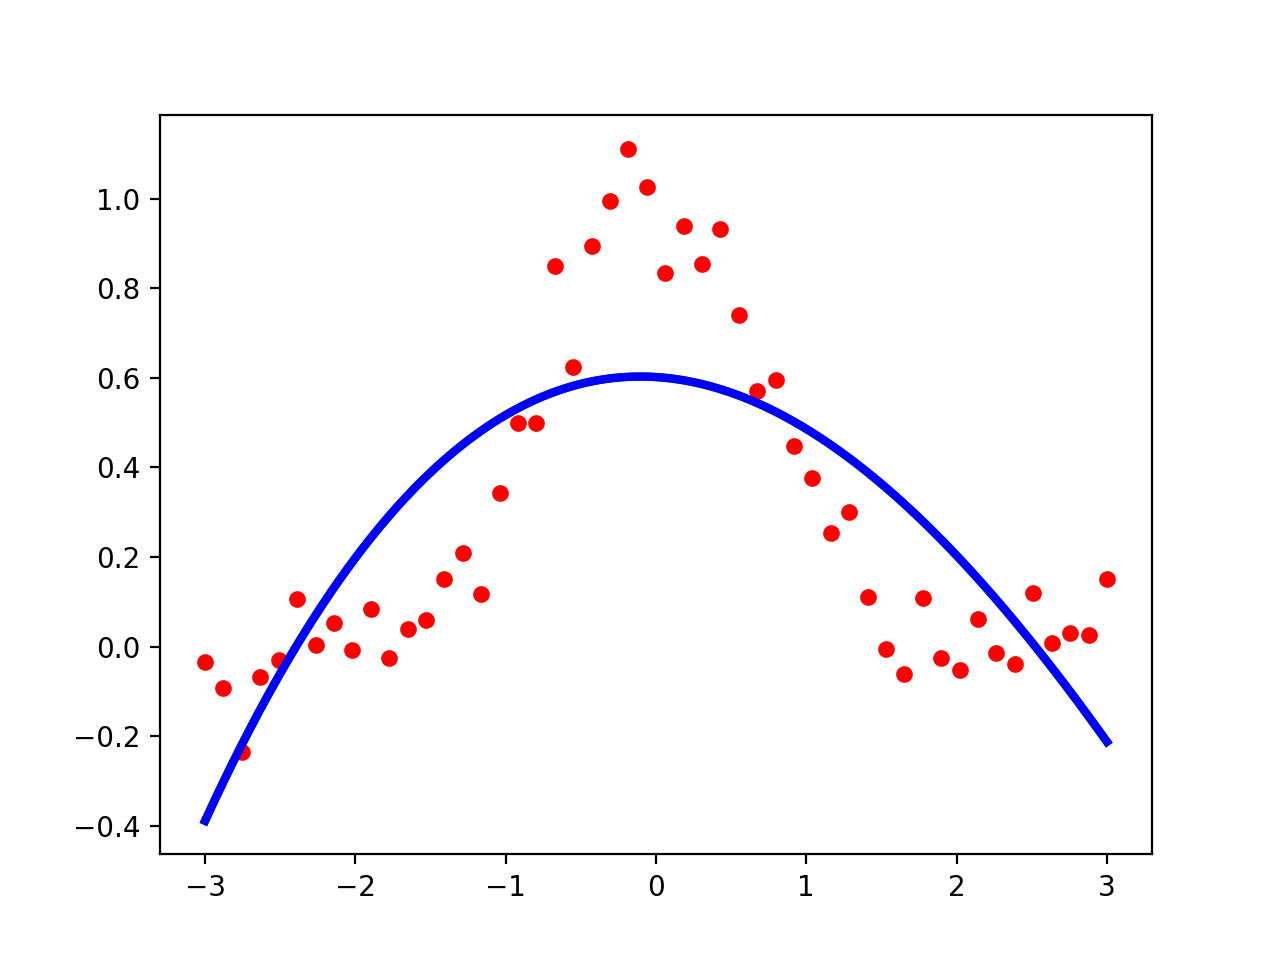
\includegraphics[width=\linewidth]{fit_ex.png}
  \caption{Example fit for Univariate BSpline Approximation}
  \label{fig:optPol1}
\end{figure}
\end{document}
